\chapter{Programação \textit{Multithread}}
Outra forma de fazer duas ou mais tarefas ao mesmo tempo é utilizado \textit{multithreads}. Conforme já discutido em sala de aula, \textit{multithreads} são diferentes linhas de execução em um processo.

Existem algumas bibliotecas para trabalhar com \textit{multithreads}. Por exemplo, a POSIX \textit{Threads} (PThreads) -- que utilizaremos neste tutorial -- e a OpenMP, cujo paradigma é diferente da PThreads.

Neste tutorial, serão utilizadas as seguintes primitivas  da biblioteca PThreads:

\begin{itemize}
\setlength{\itemsep}{1pt}\setlength{\parskip}{0pt}  \setlength{\parsep}{0pt}
\item \texttt{pthread\_create()}: responsável pela criação de uma \textit{thread}.
\item \texttt{pthread\_exit()}: responsável por retornar um valor de uma \textit{thread}.
\item \texttt{pthread\_join()}: adiciona uma barreira para aguardar por uma segunda \textit{thread}.
\item \texttt{pthread\_self()}: obtém o identificador da \textit{thread}.
\end{itemize}

Na biblioteca PThreads em particular, os \textit{threads} são implementados como funções, com uma \enquote{assinatura} específica. Essa \enquote{assinatura} é um padrão que as funções devem adotar na sua declaração, conforme ilustra a Figura~\ref{fig:assinaturaThread} a seguir. 

\begin{figure}[!htb]
    \centering
    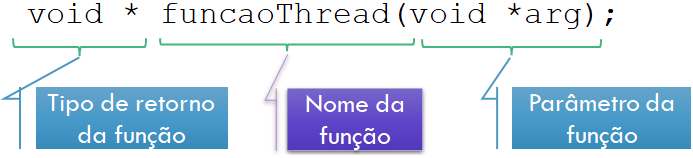
\includegraphics[width=.8\textwidth]{AssinaturaThread.png}
    \caption{Assinatura padrão de um \textit{thread}.}
    \label{fig:assinaturaThread}
\end{figure}

Note que a função que implementa um \textit{thread} deve, obrigatoriamente, retornar o tipo \enquote{\mbox{\texttt{void *}}} e receber como parâmetro um tipo \enquote{\mbox{\texttt{void *}}}. Tanto o nome da função, quanto o nome da variável passada como parâmetro pode ser definidos pelo programador.

A utilização do tipo \enquote{\mbox{\texttt{void *}}} possibilita ao programador a utilização de um endereço para qualquer tipo de dado. Contudo, para evitar que o compilador lance advertências, é preciso fazer uma conversão de tipos (\textit{cast}) para usar o conteúdo do endereço utilizado.

\section{Exemplo simples de utilização da biblioteca PThreads}
Para ilustrar a utilização da biblioteca PThreads, começaremos com um exemplo muito simples. Observe o programa \texttt{thrd.c} a seguir. O programa dispara duas \textit{threads} que \enquote{dormem} um tempo aleatório. 

Atente para os comentários que aparecem no código. Esses comentários explicam a utilização das primitivas da biblioteca PThreads.

\section*{thrd.c}
\lstinputlisting[style=MyCStyle]{./Programas/Thread/thrd.c}

A definição das funções chamadas pelo programa principal estão no arquivo a seguir.

\section*{funcoes.c}
\lstinputlisting[style=MyCStyle]{./Programas/Thread/funcoes.c}



\section{Exercício}
Compile e execute o programa anterior. Antes de compilar o programa, mude para o diretório onde se encontram os arquivos \texttt{funcoes.c} e \texttt{thrd.c} , com o seguinte comando:

\begin{lstlisting}[style=MyBashStyle]
cd ../Thread
\end{lstlisting}

Para compilar, utilize a seguinte linha de comando:

\begin{lstlisting}[style=MyBashStyle]
gcc -lpthread funcoes.c thrd.c -o thrd
\end{lstlisting}

\textcolor{orange}{\faWarning} Observação: a chave \textcolor{red}{\texttt{-lpthread}} indica que será usada a biblioteca \texttt{pthread} para Linux. Em algumas distribuições, você deve usar a chave \textcolor{red}{\texttt{-pthread}}.

\section{Passagem de parâmetros para \textit{threads}}
Vejamos agora como ocorre a passagem de parâmetros para os \textit{threads}. Antes, é preciso lembrar que na biblioteca PThreads, os \textit{threads} usam uma assinatura específica descrita na Figura~\ref{fig:assinaturaThread}. 

Para passar parâmetros para os \textit{threads}, é preciso encapsulá-los em uma estrutura e passar o endereço dessa estrutura para o \textit{thread}. Depois, já no escopo da função que implementa o \textit{thread}, esses parâmetros podem ser atribuídos às variáveis locais para serem utilizados.

\section{Retorno dos \textit{threads}}
De forma análoga à passagem de parâmetros, um \textit{thread} deve retornar um endereço de memória ou o endereço nulo (\texttt{NULL}).  

É importante destacar que, se um \textit{thread} for devolver um endereço de memória, essa posição de memória deve ter sido alocada dinamicamente. A razão para isso é que, após o término da função, todas as variáveis locais declaradas no escopo daquela função deixarão de existir. Portanto, um endereço alocado dinamicamente continuará existindo, mesmo após o término da função, até que a desalocação seja feita explicitamente (com a função \texttt{free}).

Também é preciso lembrar que esse endereço de memória devolvido ao final do \textit{thread}, precisa ser convertido para um tipo de dado específico. Caso essa operação não seja feita, o compilador poderá informar um erro de tipos na utilização da variável.

Como um exemplo de passagem de parâmetros, vejamos o exemplo a seguir. Trata-se de um programa \textit{multithread} que vai calcular a média dos números em um vetor. Nesse exemplo em particular, vamos usar um vetor de 100 posições e cada um dos quatro \textit{threads} calculará a soma parcial das suas respectivas partições (cada \textit{thread} calculará a soma de 25 elementos do vetor).

Note, logo no início da função que especifica o \textit{thread}, como os dados são extraídos do parâmetro \texttt{args} e atribuídos às variáveis locais. Essa estratégia facilita o uso posterior das variáveis na função.

Perceba também que a variável de retorno (\texttt{soma}) é um ponteiro. Esse ponteiro terá a memória alocada dinamicamente na função para que possa ser devolvida no final do \textit{thread}. 

\section*{mediaThread.c}
\lstinputlisting[style=MyCStyle]{./Programas/Thread/mediaThreads.c}

\section{Exercício}
Compile e execute o programa anterior utilizando a seguinte linha de comando:

\begin{lstlisting}[style=MyBashStyle]
gcc -lpthread auxFuncs.c mediaThreads.c -o mediaThread.o
\end{lstlisting}

\textcolor{orange}{\faWarning} Observação: a chave \textcolor{red}{\texttt{-lpthread}} indica que será usada a biblioteca \texttt{pthread} para Linux. Em algumas distribuições, você deve usar a chave \textcolor{red}{\texttt{-pthread}}.
